%http://web.mit.edu/course/21/21.guide/capitals.htm
This chapter is dedicated to the methodology that we propose to achieve the objectives of this thesis, i.e. Methodology and Algorithms for High-level Modeling of CR Impacts on Electrical Systems.




The work accomplished so far in the literature studied fault behaviors at high-level of abstraction under the assumption of fault occurrence. As discussed in Chapter~\ref{faultmodels} there is no evidence available, are these models exists for an FPGA based system? If yes, What is the probability of observing any particular fault model? How many different fault behaviors occur under the radiation experiment that lasts few hours?  What is the relationship of these faults models with the underlying hardware architecture regarding bitflips?

We would like to answer all these questions by making the HMM. The HMM helps to find the answers of all the questions mentioned above, once we get the answers of these questions, designer no longer needs to do the hardware-based experiments to find the fault behavior and particular hardware resource utilization. 

A designer can find the answer by giving the fault models, its probability of occurrence, original circuit to produce faulty components library, respective VHDL component to find resource utilization. I would like to start by giving the fault models we may get during the testing, then explain how I use HMM to solve our problem. How to make a faulty components library, its utilization will be discussed at the end of this Chapter.
\label{approach}
\section{Relation to State-of-the-Art}
Starting from the background, remember the facts established in the Chapter~\ref{introduction} mainly the fact that the digital circuits vulnerable to radiation require high-reliability requirements. The faults e.g., stuck-at-fault due to particle, strikes cause different effects in the system behavior based on an FPGA. As discussed in Chapter~\ref{related} in digital sequential circuit, a single event upset causes a multiple faulty response of the underlying circuit. Consider the example of  a 3-bit counter as shown in Figure~\ref{fig:counter}. The node is stuck-at-0$\rightarrow C_0$. This stuck node response can propagate to multiple outputs, as shown in Table~\ref{c@0-c0} and produce multiple erroneous outputs. The way this SEU interrupt at high-level of abstraction could typically manifest multiple correlated; "change in states of the design," and "change in signature values." To model the fault occurs at the low-level, and make the model of the faulty response of the circuit at high-level of abstraction, I propose to use the Hidden Markov Model. 




\begin{figure}[tb!]
 \centering
  \captionsetup{justification=centering}    
   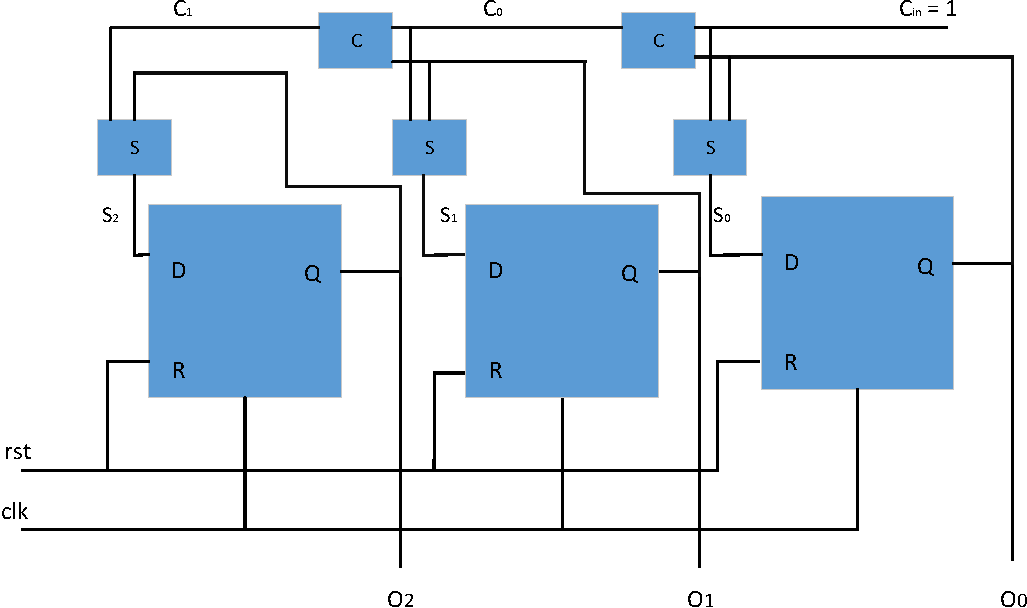
\includegraphics[scale=0.6]{Figures/counter.pdf}
   \caption{Signature Generation.}
\label{fig:counter}
\end{figure}
\begin{table}[tb!]
\center
\caption{Stuck-at-0$\rightarrow C_0$}
\label{c@0-c0}
\begin{tabular}{|c | c| c | c| } 
 \hline
 \rowcolor{lightgray}
Faulty Value(Binary) & Faulty Value & Original Value & Arithmetic Signature   \\ 
\hline
 
 
 000& 0 &0 & 0  \\
 \hline
 001 & 1 & 1 & 0 \\ 
 \hline
 
 000 & 0 & 2 & 2 \\
 \hline
 001& 1& 3& 2 \\
 \hline
 000 & 0  &  4& 4 \\
 \hline
 001 & 1 & 5 &4  \\
 \hline
 000 & 0 & 6 & 6 \\
 \hline
 001 & 1 & 7 & 6 \\
 \hline
 
 
\end{tabular}
\end{table}
\section{Description of Fault Behavior}
Before going into the details of the HMM approach, I prefer to give a brief description of fault behaviors that we may observe during the radiation testing and fault emulation. Based on the fault models mentioned in the Chapter~\ref{faultmodels} the most prominent fault behavior we will observe is "Stuck-at-fault." However, there are few other fault behaviors; we might experience which shows the limitation of the stuck-at-fault model, because these fault behaviors cannot be imitate with stuck-at-fault. We need to develop more fault models at high-level to imitate the same faulty behavior. The pseudo-codes for some high-level fault models are mentioned in the Appendix~\ref{appendix}.
\begin{itemize}
\item \textbf{Lost signal or event fault:} This kind of fault model we might observe when a certain process of a system stop working. For example, a 3-bit counter, the result of the first two bits are accurate but the third flip-flop didn't respond.

\item \textbf{Stuck Signal:} In this kind of fault model the signal is stuck to some fixed value. For example, the input of a FIR filter stuck to some unknown fixed value. 
 
\item \textbf{Variable change fault:} This fault behavior shows the situation in which either inputs, outputs, or intermediate calculations changes to some other value. Now, consider a case as shown in Table~\ref{FMFIR}, the expected faulty output of the FIR filter: $\{1, 6, 5, 16, 15\}$ due to variable change fault the faulty output observed: $\{1, 80, 5, 16, 15\}$. The signature observed from the variable change fault is only one position different from the expected signature (stuck-at-fault).  It means we cannot use the stuck-at-fault model to imitate this kind of faulty behavior. This is  the limitation of the stuck-at-fault (applies to other models as well). In this thesis will make different fault-models to represent that signature.
\begin{table}[tb!]
\center
\caption{Variable Change Fault Models FIR}
\label{FMFIR}
\scalebox{0.75}{
\begin{tabular}{|c|c|c|c|} 
 \hline
 \rowcolor{lightgray}
\shortstack {Faulty Value \\(Stuck-at-fault)} & \shortstack {Faulty Value \\ (Variable change)} & \shortstack {Signature \\ (Stuck-at-fault)} & \shortstack {Signature \\ (Variable Change)}   \\ 
\hline
 
 
 1& 1 & 0 & 0  \\
 \hline
 6 & 80 & 1 & -75 \\ 
 \hline
 
 5 & 5 & 0 & 0 \\
 \hline
 6& 16& 1& 1 \\
 \hline
 15 & 15  &  0& 0 \\
 \hline
 
 
\end{tabular}
}
\end{table}
\item \textbf{Changing the specified range of output:} This kind of faulty behavior shows if we get the output which is out of the range of the expected value. For example, the 3-bit counter gives the output that is out of the range of 3-bit counter, e,g., $out$ $<=$ $10$.
\item \textbf{Delayed Fault:} This fault model explains the situation in which the output is delayed according to the predetermined outputs. For example, the output of the counter comes after ten clock cycle delays.
\item \textbf{Invert Fault:} When the fault occurs, and it inverts the actual value, e.g., true to false and false to true. This kind of fault observes for \textit{if} and \textit{else}
conditional statements. For example, the \textit{if} statement start working on condition: \textit{false} instead of \textit{true}.

\item \textbf{Short Circuit Fault:} The fault model makes the two independent variables dependent on each other.

\item \textbf{Open Circuit Fault:} The signal can take any non-deterministic value.

\item \textbf{Stuck-Then:} This fault model describes the failure of the \textit{if-then-else} statement in which the \textit{else}
 statement never executed. In the following example, the \textit{else }
statement never execute.

\item \textbf{Stuck-Else:} This fault model represents the behavior in which the \textit{then} statement never execute.

\item \textbf{Dead Process:} This fault model describes the failure of the statement inside the \textit{process} statement.

\item \textbf{Micro-operation fault}: This fault model represents the failure of the operation of the logical operator, arithmetic operator, and relational operator, e.g., xor <=.   
\item \textbf{Swap Value Fault:} The fault model depicts swapping the values between two variables.

\item \textbf{Constant Fault}: This fault model force the variable to assign some unknown constant.

\item \textbf{Amplification}: This fault model force the variable to multiply with some value.

\item \textbf{Increase and Decrease }: This fault model force the variable either increase or decrease from its original value.
\end{itemize}



\section{Why Hidden Markov Model?}
We plan to use HMM for modeling and analysis of the sequential circuits susceptible to soft-errors. We prefer to use the HMM analysis over the other modeling techniques, e.g., BDD/ADD, Boolean Satisfiability problem (SAT), Monte-Carlo sampling, approximate approaches, symbolic methods for efficient estimation, and simulation methods. As all these techniques require to transform the circuit into their respective tool and require a lot of mathematical notations. While in HMM we can directly make the model just looking into the signature values, construct the high-level model that can be further use for the analysis. HMM can be used suitably to model systems which consist of different observable outputs (signature in our problem domain) on different hidden conditions, i.e., fault behavior, e.g., stuck-at-fault, or delay fault.
To make the HMM, we first need to have two copies of the original circuit --- named Fault-Free circuit, and a faulty circuit (\textit{hit circuit}). The Fault free circuit is used to collect the correct behavior of the circuit (fault-free outputs), and faulty is used to collect the faulty response of the circuit (faulty output). The difference between them gives us the signature as shown in Figure~\ref{fig:SG} and represented in the following equation.
\begin{center}
$Arithmetic$ $Signature$ $=$ $Original$ $Value$ $-$ $Faulty$ $Value$
\end{center}
 \begin{figure}[tb!]
 \centering
  \captionsetup{justification=centering}    
   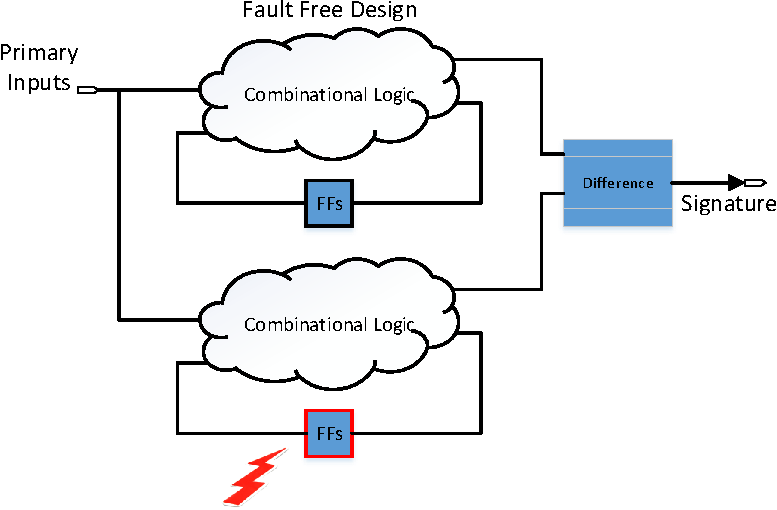
\includegraphics[scale=0.8]{Figures/signature1.pdf}
   \caption{Signature Generation}
\label{fig:SG}
\end{figure}

Hidden Markov Model is a statistical model in which a system that can be modeled is assumed to be a Markov process with unobserved states, i.e., hidden states. A Markov process  is a stochastic process that satisfies the Markov property -- \underline{memorylessness}, meaning, a process that satisfies the Markov property, if the prediction of the future of the system's output based solely on its present state, it is independent of the future and past states. In order to apply the HMM, we need a system that generates probabilistic output patterns in time, e.g., faulty response of the 3-bit counter. Afterwards, we need to look at the system and need to know which states of the system give that particular output ---  the underlying system is hidden. For example, in the case of a 3-bit counter, the observed sequence is the "signature" and the hidden is the "stuck-at-fault or any other fault." Now, we wish to devise a model to predict that "fault behavior", without actually knowing about the fault. 

In the 3-bit counter example we  get   different signatures. Here for simplicity, I give the example of four different signatures and construct the HMM. The signatures are: \textit{Sign-1, Sign-2, Sign-3, and Sign-4}. The observed signatures are probabilistically related to the hidden process. We can model such process using a Hidden Markov model, where there is an underlying Hidden Markov process changing over time, and a set of observable states which are related to somehow to the Hidden states.
The figure~\ref{fig:HMM-3-bit} shows the Markov model for the hidden and the observable states for the 3-bit counter example. The hidden states are (stuck-at-fault, delay fault, and variable change), and observable states are  the signatures. 
\begin{figure}[tb!]
 \centering
  \captionsetup{justification=centering}    
   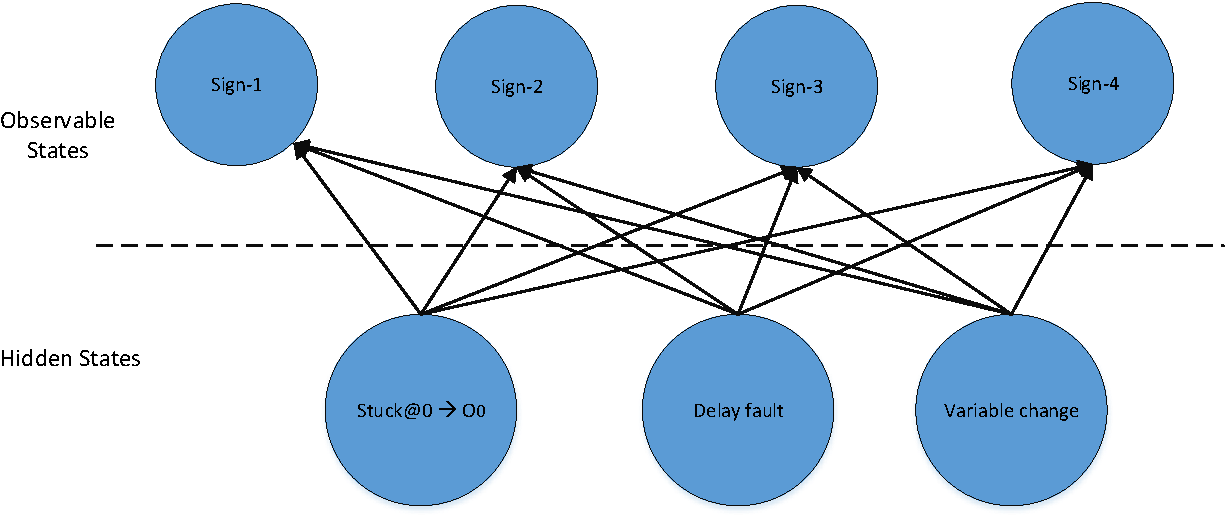
\includegraphics[scale=0.8]{Figures/HMM.pdf}
   \caption{HMM model 3-bit counter.}
\label{fig:HMM-3-bit}
\end{figure}

HMM is based on  two things: a) Observable States, and b) Hidden States. If we closely observe above mentioned 3-bit counter example, we realized that in this scenario --  signatures are the observable state, and the faults occurs due to the bit-flip are the hidden states. In this thesis, we used the concept of HMM to construct the high-level model based on the signature information.

\section{Modeling Hidden Markov Model}
\begin{figure}[tb!]
 \centering
  \captionsetup{justification=centering}    
   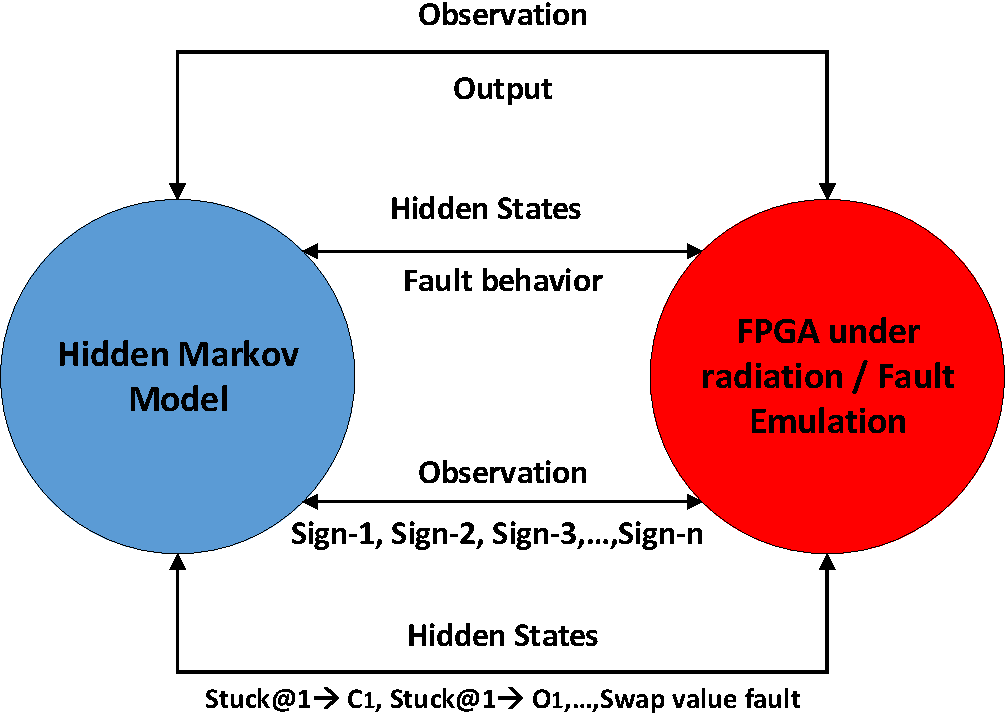
\includegraphics[scale=0.8]{Figures/HMM-air.pdf}
   \caption{Hidden Markov Model to the FPGA based fault emulation system}
\label{fig:HMM-air}
\end{figure}
The Figure~\ref{fig:HMM-air} shows the basic HMM applied to the FPGA based fault emulation system. We can model this system with the HMM, where, the outputs emitted by the system (FPGA under radiation/ Fault Emulation) are observable (signatures --- in our problem domain), and underlying states of the system (Stuck-at-fault, delay fault, swap value fault, etc.). HMM can be visualized as a simple finite state machine. The HMM has a strong statistical foundation; it has the ability for efficient learning algorithms, which can take place directly from the raw sequence data. \textbf{The problem in hand} can be solved by using the HMM as we can observe the sequence of signatures, but we do not know  which fault behavior  of the system it went through to generate that particular signature. Because we don't know which node is attached by the SEU during the radiation experiment or the fault injection. The analyses of Hidden Markov Model seek to recover the states from the observed data.


\subsection{Probabilities in a HMM}
There are three important things to know about the probabilities in HMM.
\begin{itemize}
\item The connections between the hidden states of the system, and the observable states of the system represent the probability of generating a particular observed state given that the Markov process is in a particular hidden state as shown in Figure~\ref{fig:HMM-3-bit}.
\item The probabilities entering into the observable states will sum to "1." 
\begin{center}
$Pr(Sign-1|Stuck) + Pr(Sign-1|delay) + Pr(Sign-1|variable $ $ change)  = 1 $
\end{center}
\item In addition, probabilities define the Markov process, we have another matrix termed as "confusion matrix", which contains the probabilities of the observable states given a particular hidden state. The following matrix is the confusion matrix for the 3-bit counter example. We can extract the confusion matrix values from the radiation and fault emulation experiment.
\begin{center}
CM = \bordermatrix{~& Sign-1 & Sign-2 & Sign-3 & Sign-4\cr
                  Stuck@0\rightarrow{C_0}& 0.60 & 0.20 & 0.15&0.05 \cr
                  $Delay$   & 0.25 & 0.25 &0.25 &0.25\cr
                  $Variable$ $ $ $Change$ & 0.05 & 0.10 &0.35 &0.50\cr}
\end{center}
\end{itemize}
\subsection{HMM Parameters}
A hidden Markov Model is described as $ \Pi = \{\pi, A, B\}$ as shown in Figure~\ref{fig:MARKOV-SERIS}, where,
\begin{figure}[tb!]
 \centering
  \captionsetup{justification=centering}    
   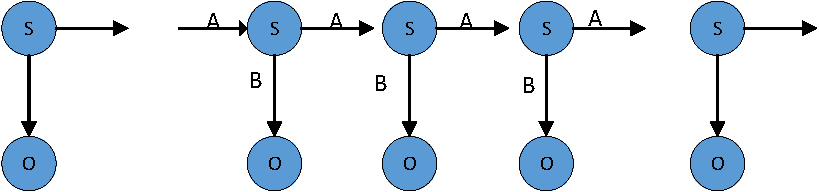
\includegraphics[scale=0.8]{Figures/MARKOV-SERIS.pdf}
   \caption{HMM Formalization.}
\label{fig:MARKOV-SERIS}
\end{figure}
 $(\pi) = $ initial state probabilities vector; 

$A = (a_ij)$ state transition matrix;  \hspace{0.3cm} $P_r(x_i | {x_j}_{t-1})$


$B = (b_ij)$  confusion matrix;     \hspace{0.3cm}        $P_r(y_i | x_j)$ 


We can find the initial state probability vector, state transition matrix and confusion matrix  from our experimental data generated by the radiation or emulation experiment.
\textbf{Hidden States:} The true states of the system that may be described by a Markov Process, e.g., stuck-at-fault, etc.,
\textbf{Observable State:} The state of the process, visible, e.g., Signature.
\textbf{$\Pi$ $Vector$:} contains the probability of the hidden model being in a particular hidden state (fault behavior) at the time t = 1.
\textbf{State transition matrix:}  holding the probability of a hidden state given the previous hidden state.
\textbf{Confusion matrix:} containing the probability of observing a particular observable state given that the hidden model is in a particular hidden state. 
Once we model a system with HMM, it helps to find three problems. We model them according to our problem, i.e.,
\begin{tcolorbox}[width=\textwidth,colback={gray},title={Evaluation },colbacktitle=gray,coltitle=black]  
Find the probability of an observed signature given an HMM.  
\end{tcolorbox}
\begin{tcolorbox}[width=\textwidth,colback={gray},title={Decoding },colbacktitle=gray,coltitle=black]  
Finding the hidden states (fault models) that most probably generated an observed sequence. 
\end{tcolorbox}
\begin{tcolorbox}[width=\textwidth,colback={gray},title={Learning },colbacktitle=gray,coltitle=black]  
The third problem is generating an optimized HMM given a sequence of signatures (observations).
\end{tcolorbox}
\section{HMM Application for Signature}
Hidden Markov Model can give the answer to three major questions that we can use in our problem domain. It helps to a) compute the probability of a given sequence of signatures, b) compute the most probable sequence of states, and c) given a sequence of observations and learn the best HMM model.
In order to find the solution of these three questions, we called it HMM applications.
\textbf{The Three basic HMM Applications are:}
\begin{itemize}
\item Application 1 : Probability Evaluation
 \begin{itemize}
 \item How do we efficiently compute $P(O|\Pi)$ the probability of the signatures given that the HMM parameters from the given observed signature sequence $O = {O_1, O_2,...,O_n}$.
 
  \begin{itemize}
  \item We can use the forward algorithm~\cite{ghahramani1996factorial}.
  \end{itemize}
 \end{itemize}
\end{itemize}
\begin{itemize}
\item Application 2 : Optimal State Sequence
 \begin{itemize}
 \item Given signatures sequence $O = {O_1, O_2, ...., }O_n$ and model $\Pi$ how we choose a hidden state sequence (stuck-at-fault, variable change fault, etc.) $Q={q_1,q_2,q_3, ..., q_n}$
that is optimal, i.e., best explains the data. 
  \begin{itemize}
  \item Viterbi algorithm~\cite{forney1973viterbi} helps to find the answer to this application.
  \end{itemize}
 \end{itemize}
\end{itemize}
\begin{itemize}
\item Application 3 : How do we adjust the parameters of the model $\Pi = \{\pi, A, B\}$ to maximize the likelihood $P(O|\Pi)$ 
 \begin{itemize}
 \item Given observation sequence $O = {O_1, O_2,....,} O_n$ adjusting the hidden HMM parameters $ \Pi = \{\pi,A, B\}$ to maximize the probability $P(O|\Pi)$ 
  \begin{itemize}
  \item The solution is either to use Expectation-Maximization~\cite{moon1996expectation} or Baum-Welch’s re-estimation~\cite{leggetter1995maximum}.
  \end{itemize}
 \end{itemize}
\end{itemize}


\subsection{Evaluation Application}
For probability evaluation, we need to compute the likelihood of an observed signature sequence $O = {O_1, O_2,...,O_t}$ given a particular HMM model $ \Pi = {\pi, A, B}$. The computation of this probability involves all the possible hidden state sequence and evaluate the corresponding probability. 
\begin{itemize}
\item  $P(O | \Pi) = \sum\limits_{\forall Q}^{} P (O | X, \Pi) P (X, \pi)$ 
\item For a specific state sequence $X = {x_1, x_2,...,x_t}, P(O | Q, \Pi):$


 $P (O | X, \Pi) = \prod_{t=1}^{T} P (o_t | q_t, \Pi) = \prod_{t=1^{T} b_{x_t} (o_t)}$
 
 \item The probability of the state sequence $X$:
 \\
 \hspace {0.2cm} $ P (X | \Pi ) = \pi_{x_1} a_{x_1 x_2} a_{x_2 x_3},...,a_{x_{T-1} x_T}$
 
 \item The final expression we get:
 
$P (O | \Pi ) = \sum\limits_{x_1, x_2,..., x_T} \pi_{x_1} b_{x_1} (o_{x_1}) a_{x_1 x_2} b_{q_2} (o_{x_2}),..., a_{x_{T-1} x_T} b_{xT} (o_{xT})$
\item If there are $N^T$ possible state sequence, this approach becomes infeasible to apply or implement even for the smallest circuits.
\begin{itemize}
\item For N = 5 and T = 100, the order of magnitude --- $10^7$
\end{itemize}
 
\end{itemize}
This problem can be solved by using the Forward Algorithm:
\textbf{Example:} Consider an example where we have a number of HMMs (a set of triplets $(\pi, A, B)$) describing different systems, and a sequence of observation, i.e., you will get this system by performing radiation/fault emulation experiments for hours of testing. You have a number of HMMs constructed in the Simulink library and want to know which HMM most probably generated given sequence (signature).
We will use the forward algorithm to calculate the probability of an observation sequence given a particular Hidden Markov Model, and find the most probable HMM. Suppose that you have an HMM that describes the fault behavior, and we also have a sequence of signatures. Suppose the fault behavior works in this order $(stuck-at-c_0)$, delay fault, dead process, the signatures: Sign-1, Sign-2, and Sign-3. There is some hidden relationship between fault behavior and the signatures, we can make a "Trellis" diagram as shown in Figure~\ref{fig:trellis}
\begin{figure}[tb!]
 \centering
  \captionsetup{justification=centering}    
   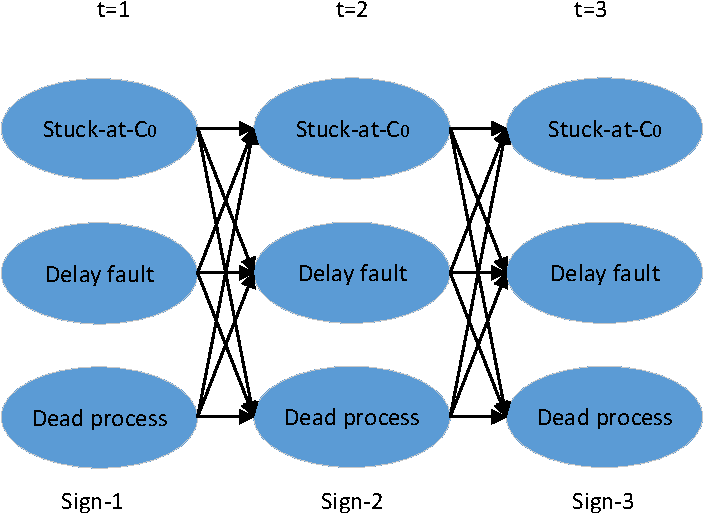
\includegraphics[scale=0.8]{Figures/viterbi.pdf}
   \caption{Trellis Diagram}
\label{fig:trellis}
\end{figure}
From the trellis figure we conclude the following:
\begin{itemize}
\item Each column in the trellis represents the possible state of the fault behavior and each state in the column is connected to the each state in the adjacent column.
\item The transition between the states --- state transitions has the probability provided by the "state transition matrix."
\item Each column in the signature observations at that time: the probability of this signature observation given any one of the above fault behavior states is provided by the confusion matrix. 
\item As mentioned above one of the possibilities of calculating the probabilities of the observed states would be finding each possible sequence of the hidden fault behavior states and sum all these probabilities. Just for this example, there would be $3^3 = 27$ possible sequences, it’s extremely complex to do this. So, we will propose to use the forward algorithm that can calculate the probabilities of observing a sequence recursively given HMM.
\end{itemize}
\textbf{Forward algorithm Steps:}
We need to calculate the probability of observing a signature recursively given HMM. 
\begin{enumerate}
\item The first step is the initialization step at t = 1 when there is no path to the state. The probability of being at state at t = 1 is actually the initial probability:
\begin{itemize}
 \item $P (state | t = 1) = \pi $
\item The initial probability at t = 1 is the probability multiplied by the associated observation probability.
$\alpha(j) = \pi(j) b_i (O_1)$
\end{itemize}
\item Second, we need to define a \textbf{partial probability} which is the probability of reaching an intermediate state in the trellis.
\begin{itemize}
\item For example, the T-long signature sequence: $(Y_k1, Y_k2,..., Y_kT)$, partial probabilities $\alpha 's$. Figure~\ref{fig:trellis} shows the Trellis diagram. Calculate the probability of reaching an intermediate state in the trellis diagram as the sum of all possible paths to that state.
\item The partial probability of state $j$ at time $t$ is $t(j)$, to calculate the partial probability:
$\alpha_t(j) = P (observation $ $ | $ $ hidden state $ $ is $ $ j) \times P (all $ $ paths $ $ to $ $ state  $ $ j $ $ at $ $ time $ $ t)$
\item The partial probabilities for the final observation hold the probability of reaching those states going through all the possible paths. The sum of these final partial probabilities is the sum of all possible paths. 
\hspace {4.5 cm}

$\alpha_{t+1}(j) = b_jk_{t+1} \sum\limits^{n}_{i = 1} \alpha_t(i) a_{ij}$

\end{itemize}
\item This expression can be used to calculate the $\alpha$. We can find the probability of an observation given HMM. The probability of the sequence given the HMM is then the sum of the partial probabilities at time t = T.
 
 \hspace {4.5 cm}$P(Y^K) = \sum\limits^{n}_{j=1} \alpha_T (j)$
\end{enumerate}

\subsection{Decoding Application}
\begin{figure}[tb!]
 \centering
  \captionsetup{justification=centering}    
   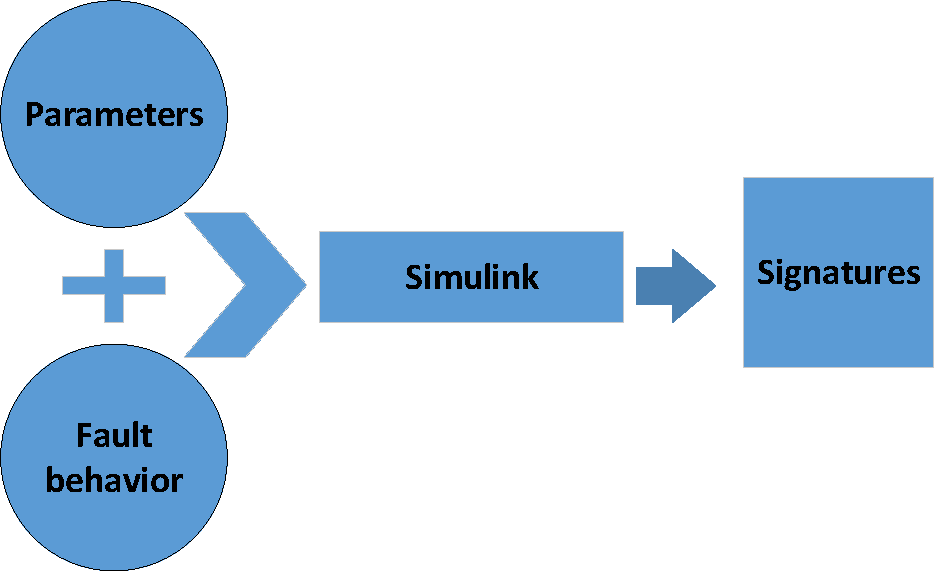
\includegraphics[scale=0.8]{Figures/fromhiddentosignature.pdf}
   \caption{Fault behavior to Signatures}
\label{fig:HMMsig}
\end{figure}
To design it for the decoding application there are two possibilities to use either Viterbi decoding algorithm or  posterior decoding. The Viterbi gives the most likely sequence while posterior decoding gives the most likely state at each position. Here, we are more focused on the sequence of hidden states (use in simulators to reproduce the signatures) that give the respective signatures, in this case Viterbi algorithm is preferable. The decoding capability of HMM helps to find the sequence of the fault behavior whether it comes only from the stuck-at-fault and/or other fault behavior that generated the given signatures. In the FPGA fault emulation and radiation experiment we are interested to find the fault behavior of the system as they represent some valuable information that can later be used to give to the Simulink model to reproduce the signatures (if we know the fault behavior and their respective probabilities) as shown in Figure~\ref{fig:HMMsig}.

 
\textbf{Example:} Consider an example of the signature and stuck-at-fault; an FPGA test designer can only sense the signature but wants to know the fault behavior to make the high-level model based on this information.


\textbf{Answer}: We will use the \underline{Viterbi Algorithm} to determine the most probable sequence of fault behavior by giving the sequence of signatures and HMM. Inshort, decoding helps to find the hidden sequence most likely to have generated a sequence of observation --- solved using Viterbi algorithm as shown in Figure~\ref{fig:HMMsig-Vit}. 
\begin{figure}[tb!]
 \centering
  \captionsetup{justification=centering}    
   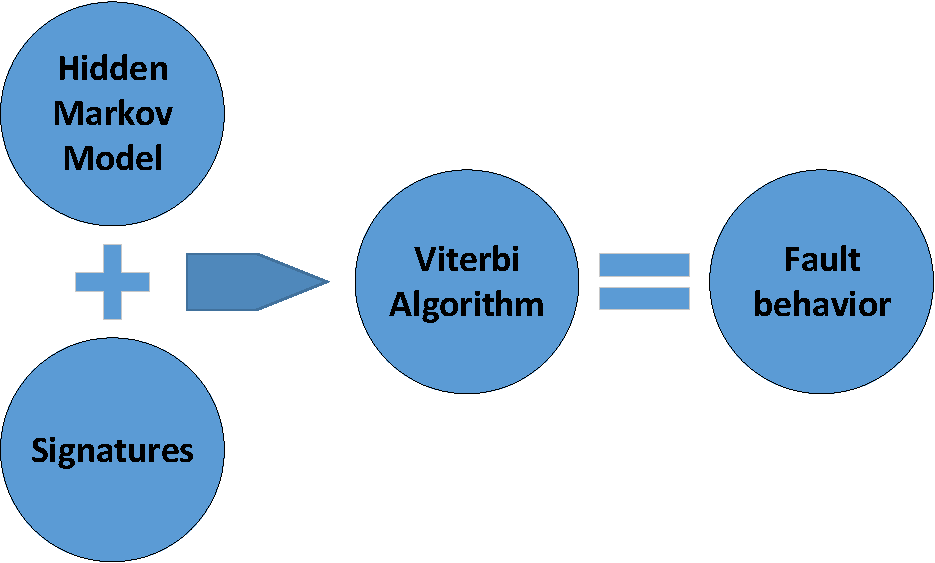
\includegraphics[scale=0.8]{Figures/HMM-plus-viterbi.pdf}
   \caption{Signatures to Fault model}
\label{fig:HMMsig-Vit}
\end{figure}
\subsubsection{Viterbi Algorithm}
The Viterbi algorithm is based on the assumption that the most \textit{likely} path (hidden states sequence), $Q^* = argmax_Q P(Q|O) $, is a good estimation of the sequence of hidden states that generated the observed sequence $(O)$. Viterbi algorithm generates a path $X = (x_1, x_2,...,x_T)$, which is a sequence of states $x_n \in S = {s_1, s_2,...,s_k}$ that produce the sequence of observations $Y = (y_1,y_2,...,y_T) \in {1,2,...,N}^T N$ $=$ $Observation$ $space$.


\textbf{Steps to apply Viterbi}
\begin{itemize}
\item Observation space $O =  {o_1,o_2,...,o_N}$
\item state space $S = {s_1,s_2,...,s_K}$
\item an array of the initial probabilities $\Pi = (\pi_1, \pi_2,...,\pi_K)$; $\pi_i$ $is$ $the$ $probability$ $the$ $x_1$ $==$ $s_i$
\item a sequence of observations $Y = (y_1,y_2,...,y_T)$; $yt == i$ observation at the time $t$ is $o_i$
\item the state transition matrix $A_ij$ stores the transition probability from state $s_i$ to $s_j$
\item emission matrix $B_ij$ stores the probability of observing $o_j$ from the state $s_i$
\end{itemize}  
\textbf{Recursion:}
We need to determine the hidden states by calculating $P(X|O)$. However, this brute force approach becomes intractable if the number of state gets larger, as the number of state path grows exponentially $(N^T)$. So, we need to calculate the $argmax_X P(X|O)$ . The most likely sequence is given by the recursion relations.
\begin{center}
\begin{itemize}
\item $V_1,k = P (y_1|k) \times \pi_k$
\item $V_t,k = max_{x \in S} (P (y_t|k) \times a_x,k \times V_t-1,x)$
\item $V_t,k$ probability of the most probably sequence $P (x_1, x_2,...,x_T, y_1,y_2,...,y_T)$
\end{itemize}
\end{center}
\textbf{Final:}
The most likely hidden state sequence $X = (x_1,x_2,...,x_N)$ 
\subsection{Learning}
The third application of the HMM is optimizing the parameters of the model. There are two possible solutions to this problem either to choose supervised learning and unsupervised learning.  In supervised learning, you have one input variable, one output variable, and use the algorithm to learn the mapping from the input to output, e.g., logistic regression, linear regression. If we  map our problem to supervised learning, in this case, our goal is to find the mapping function. In this case, whenever we have a new signature, the mapping function can predict the fault model. Now, consider a situation where only signature data is available and no information how these signatures come from the fault model.  This is the unsupervised learning because there is no answer available. In this thesis problem, we opt for the unsupervised learning, because we have only the data available that is a signature, and we will find the parameters that maximize the probability of the hidden sequence (fault models).  
We can also find the optimal solution for our model by using the learning application of the HMM. The learning application works on the model parameters and observations to find the model that fits the data. There are three different techniques to do: a) Maximum Likelihood Estimation, b) Viterbi Training, and c) Baum  Welch = Forward-Backward Algorithm. 
Suppose we have a HMM: $\Pi = (\pi, A, B)$. The Baum-Welch algorithm is used to find  a local maximum for $\Pi^* = arg max_{\Pi} P (O | \Pi)$, i.e., the HMM parameters $\Pi$ that maximize the probability of the observation.
The Baum-Welch works in the following way:
\begin{enumerate}
\item Find the forward probabilities with the forward algorithm.
\begin{itemize}
\item $\alpha_{i}(1) = \pi_{i} b_{i} (o_{1})$
\item $\alpha_{i}(t + 1) = b_{i}(o_{t+1}) \sum\limits^{N}_{j=1}\alpha_{j}(t)a_{ji}$
\end{itemize}
\item Find the backward probabilities with the backward algorithm.
\begin{itemize}
\item $\beta(t) = P(o_{t+1} o_{t+2},...,o_{T} | x_{t} = i, \Pi) $
\item $\beta_{i}(T) = 1$
\item $\beta_{i}(t) = \sum\limits^{N}_{j=1} a[x_i, x_j] b[x_j,o_{t + 1}\beta_{j}(t + 1)]$
\end{itemize}
\item Find the probability of state $i$ at time $t$.
\begin{itemize}
\item $P (x_t = i, O | \Pi) = P (o_1, o_2,...,o_t, x_t = i | \Pi) P (o_{t + 1}, o_{t + 2},...,o_{T} | x_{t} = i, \Pi) == \alpha_{i}(t) \beta_{i}(t) $
\item use the Bayes Theorem:
$P(x_t = i | O, \Pi) = \frac{P(x_t = i, O | \Pi)}{P(O | \Pi)} = \Upsilon_{i}(t)$
\end{itemize}
\item Find the probability of a transition from state $i$ to state $j$ at time $t$.
\begin{itemize}
\item $\xi_{t}(i,j) = P (x_t = i,x_{t + 1} = j | O, \Pi)$
\item These probabilities can be computed bu using the forward and backward variables:
$\xi_{t}(i,j) = \frac{\alpha_i (t) a[x_i x_j] b[x_j,o_{t + 1}] \beta_j (t + 1)   }{P(O | \Pi)}$
\end{itemize}
\item Find the expected transition and emission counts:
$\sum\limits_{t = 1}^{ T } \Upsilon_i (t)$ = expected number of transition from $x_i$
$\sum\limits_{t = 1}^{ T} \xi_t (i ,j)$ = expected number of transition from $x_i$ to $x_j$
\item Perform the parameter estimation by the ratio of expected count the maximization step:
$\overline{a}[x_i, x_j] = \frac{\sum\limits_{t = 1}^{T - 1}\xi_{t} (i, j)}{\sum\limits_{t = 1} T - 1 \Upsilon_{j}(t)} $

$\overline{b}[x_i, o_k] = \frac{\sum\limits_{t = 1}^{T - 1}\Upsilon_{j} (t) 1 (o_t = k)}{\sum\limits_{t = 1}^{T - 1} \Upsilon_{j}(t)} $
\item Stop the computation when the change in the log likelihood is smaller than a given threshold or the maximum iterations are passed.
\end{enumerate} 



\section{Faulty Components Library Utilization}
Once we have all the information about the HMM parameters, probabilities, fault models, a sequence of the hidden states. This information helps us to find the library of the faulty components. These components can be used by the designer to observe the faulty behavior of each sub-circuit on the system as shown in Figure~\ref{fig:lib1}.  If we want to find the faulty behavior of a MAC affected by the faulty behavior of an adder and/or an accumulator, we can observe this behavior by replacing the fault-free model with the faulty model.
 
\begin{figure}[tb!]
 \centering
  \captionsetup{justification=centering}    
   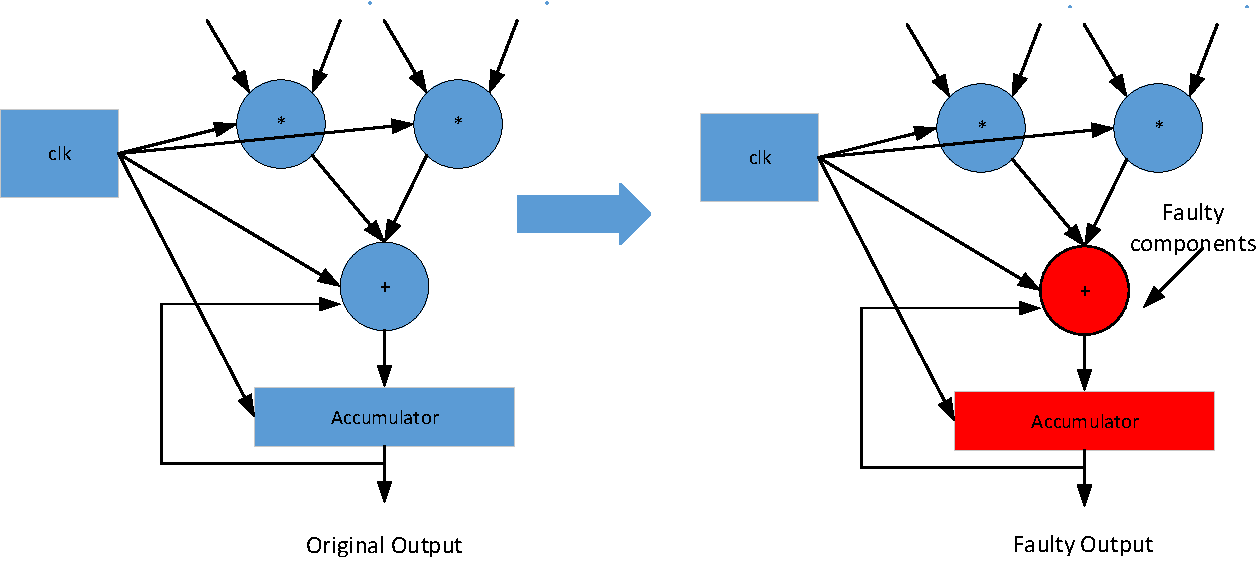
\includegraphics[scale=0.6]{Figures/MAC.pdf}
   \caption{Example of the faulty Component.}
\label{fig:lib1}
\end{figure}

We also have a plan to create a faulty finite state machines / faulty circuit models in Simulink. Then use the available functionality in the Simulink ( VHDL code generator) to find the respective VHDL entity, to get the individual VHDL entity as shown in Figure~\ref{fig:library1}. The VHDL entity helps to find the resources utilization of FPGA, and it is independent of the tool and technology easily portable to any FPGA as discussed in the Chapter~\ref{faultmodels} due to change in the tools some of the work became ineffective or out-of-date. If we have the faulty VHDL components, they are highly useful for understanding the system's behavior.


In short, we start developing the HMM from the Signatures. Then HMM helps to find the fault models associated with that particular circuit. We apply these fault models to an original circuit, make their faulty FSM / faulty circuit models, generate corresponding VHDL entity to measure the resource utilization.
%\textbf{Example:} A simulink designer needs to estimate the resource utilization of any digital circuit (operates in the radiation environment) that contain adder, multiplier, and flip-flops. He also interested to find the faulty behavior of this circuit. 
%
%A designer has a HMM which helps to find the possible fault models, based on this fault model example, designer will create the respective faulty circuit model / FSM. Once the designer have a FSM, he will create the VHDL entity and find the respective faulty circuit resource as well.tem's behavior.
%
\begin{figure}[tb!]
 \centering
  \captionsetup{justification=centering}    
   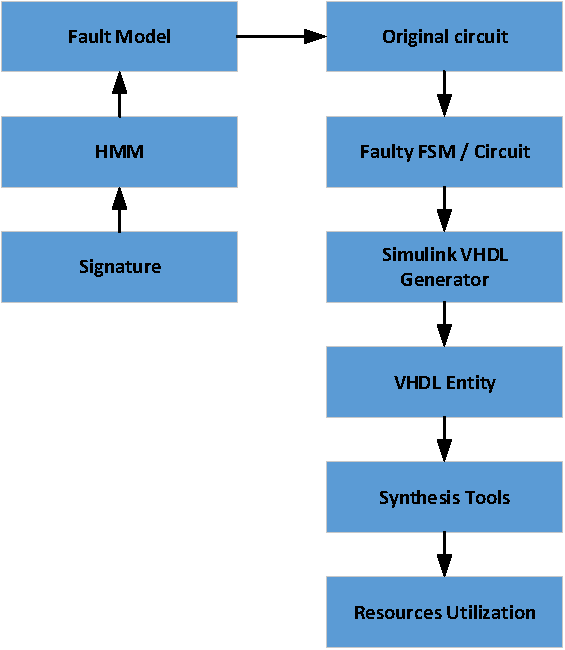
\includegraphics[scale=0.8]{Figures/library.pdf}
   \caption{VHDL entity creation and usage.}
\label{fig:library1}
\end{figure}

%
%\begin{figure}[tb!]
%
% \centering
%  \captionsetup{justification=centering}    
%   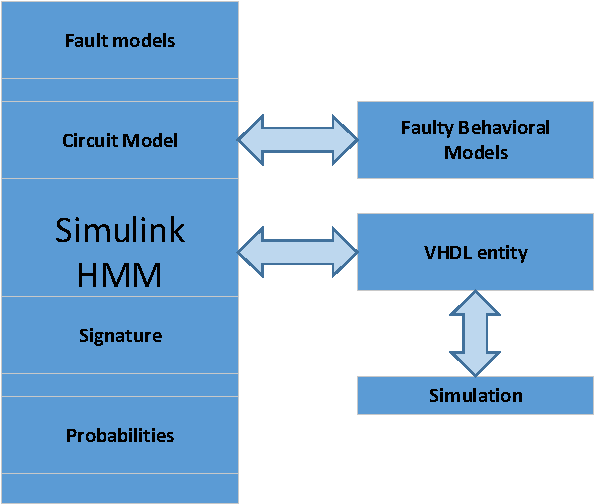
\includegraphics[scale=0.8]{Figures/simulink.pdf}
%   \caption{Library creation}
%\label{fig:lib}
%\end{figure}
%\begin{itemize}
The key utilization of this work:
\begin{itemize}
\item This work facilitates the fault simulation of faulty behavioral models. We put a fault-free circuit in Simulink based simulators and N fault models then it produces the N-faulty behavioral models.
\item We also produce the faulty VHDL entities which help to investigate the verification and testing.
\item This work able to analyze the multi-cycle error propagation behavior.
\item We will get the real-time fault occurrences and propagation data rather than user supposed fault probability distribution, e.g., normal, exponential, Poisson, Weibull, etc.
\item We will be able to study hardware faults at high-level of abstraction.
\item We will also be able to establish a relationship between the bit-flip information to the fault model.
\end{itemize}

\section{Project Plan}
\textbf{Summary} \\
\textbf{Phase  01:} The emulation platform will be the starting point of the research. We will use the sensitivity aware bit-flip technique for the configuration memory upsets. Selection of a suitable benchmark, which is probably ITC'99~\citep{ITC} used for the testing purpose and signature generation.\\
\textbf{Phase  02:} Evaluate the radiation-based experimental results for signature under the neutron radiation at Triumf.\\
\textbf{Phase 03:} Implement the above-mentioned methodology and high-level model for soft-error of the sequential circuits.